% TikZ/PGFPlots figures derived from robustness_quantum_delay_study.csv
%
% Suggested preamble additions in the manuscript:
% \usepackage{tikz}
% \usepackage{pgfplots}
% \pgfplotsset{compat=1.18}
%
% The figures below are provided as direct tikzpicture blocks so they can be
% pasted into the manuscript without requiring external CSV loading.

% ---------------------------------------------------------------------------
% Figure 1: Baseline delay trend in the OCTA benchmark
% ---------------------------------------------------------------------------
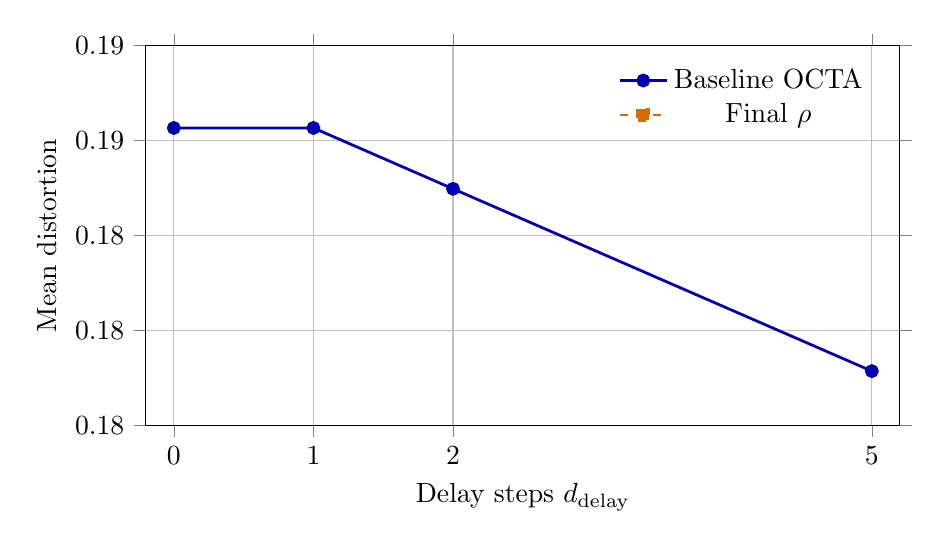
\begin{tikzpicture}
\begin{axis}[
    width=0.92\linewidth,
    height=6.4cm,
    xlabel={Delay steps $d_{\mathrm{delay}}$},
    ylabel={Mean distortion},
    xmin=-0.2, xmax=5.2,
    ymin=0.182, ymax=0.186,
    xtick={0,1,2,5},
    yticklabel style={/pgf/number format/fixed},
    grid=major,
    legend style={at={(0.97,0.97)},anchor=north east,draw=none,fill=none},
    tick align=outside,
]
\addplot[
    color=blue!70!black,
    mark=*,
    line width=1.0pt
] coordinates {
    (0,0.1851328774)
    (1,0.1851328774)
    (2,0.1844912566)
    (5,0.1825694748)
};
\addlegendentry{Baseline OCTA}

\addplot[
    color=orange!85!black,
    mark=square*,
    line width=1.0pt,
    dashed
] coordinates {
    (0,0.0965219848)
    (1,0.0965219848)
    (2,0.0961937737)
    (5,0.0959561213)
};
\addlegendentry{Final $\rho$}
\end{axis}
\end{tikzpicture}

% ---------------------------------------------------------------------------
% Figure 2: Topology comparison under the delay sweep
% ---------------------------------------------------------------------------
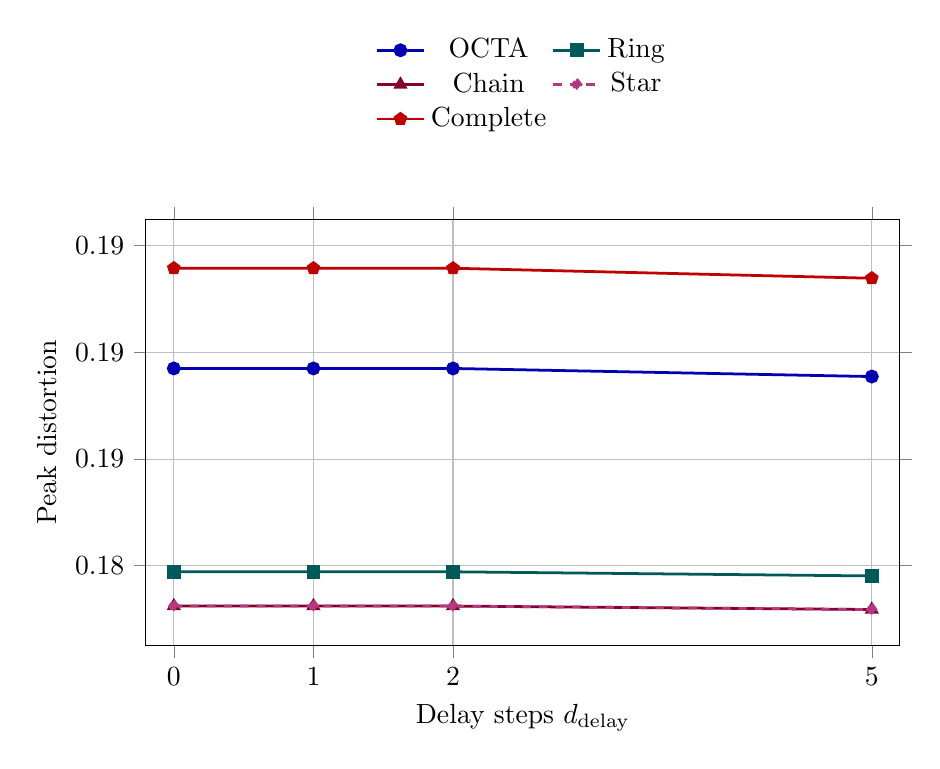
\begin{tikzpicture}
\begin{axis}[
    width=0.92\linewidth,
    height=7.0cm,
    xlabel={Delay steps $d_{\mathrm{delay}}$},
    ylabel={Peak distortion},
    xmin=-0.2, xmax=5.2,
    ymin=0.1825, ymax=0.1905,
    xtick={0,1,2,5},
    yticklabel style={/pgf/number format/fixed},
    grid=major,
    legend columns=2,
    legend style={at={(0.5,1.18)},anchor=south,draw=none,fill=none},
    tick align=outside,
]
\addplot[color=blue!70!black, mark=*, line width=1.0pt] coordinates {
    (0,0.1876994493) (1,0.1876994493) (2,0.1876989569) (5,0.1875471607)
};
\addlegendentry{OCTA}

\addplot[color=teal!70!black, mark=square*, line width=1.0pt] coordinates {
    (0,0.1838863658) (1,0.1838863658) (2,0.1838861139) (5,0.1838084933)
};
\addlegendentry{Ring}

\addplot[color=purple!70!black, mark=triangle*, line width=1.0pt] coordinates {
    (0,0.1832437579) (1,0.1832437579) (2,0.1832435472) (5,0.1831786215)
};
\addlegendentry{Chain}

\addplot[color=magenta!70!black, mark=diamond*, line width=1.0pt, dashed] coordinates {
    (0,0.1832437579) (1,0.1832437579) (2,0.1832435472) (5,0.1831786215)
};
\addlegendentry{Star}

\addplot[color=red!75!black, mark=pentagon*, line width=1.0pt] coordinates {
    (0,0.1895788638) (1,0.1895788638) (2,0.1895782552) (5,0.1893906333)
};
\addlegendentry{Complete}
\end{axis}
\end{tikzpicture}

% ---------------------------------------------------------------------------
% Figure 3: One-at-a-time sensitivity at d_delay = 5
% ---------------------------------------------------------------------------
\begin{tikzpicture}
\begin{axis}[
    width=\linewidth,
    height=8.0cm,
    xbar,
    xmin=0.18, xmax=0.279,
    xlabel={Peak distortion at $d_{\mathrm{delay}} = 5$},
    symbolic y coords={
        time step low,
        time step high,
        feedback low,
        feedback high,
        dephasing low,
        dephasing high,
        tolerance loose,
        tolerance tight,
        geometry soft,
        geometry strong
    },
    ytick=data,
    y dir=reverse,
    grid=major,
    tick align=outside,
    nodes near coords,
    nodes near coords align={horizontal},
]
\addplot[
    fill=blue!35,
    draw=blue!70!black
] coordinates {
    (0.1838084933, time step low)
    (0.1948191417, time step high)
    (0.1875471607, feedback low)
    (0.1875471607, feedback high)
    (0.1875471607, dephasing low)
    (0.1875471607, dephasing high)
    (0.1875471586, tolerance loose)
    (0.1875471607, tolerance tight)
    (0.0968922418, geometry soft)
    (0.2782020796, geometry strong)
};
\end{axis}
\end{tikzpicture}
